%----------------------------------------------------------------
% Preamble
%----------------------------------------------------------------
\documentclass[12pt, xcolor=dvipsnames]{beamer} 			         % Document class
% \documentclass[12pt,xcolor=dvipsnames,handout,notes=show]{beamer}	  % For printing
\input{../Settings/packs_beamer}   		  % Packages
%% Personalized Macros
% Definitions, Equations, Table of Contents, Tables, Subcaptions, Paths, Text Fomats

%-------------------------------------------------------------------
% Variable Definitions
%-------------------------------------------------------------------
\providecommand{\tnr}{n}
\providecommand{\tnrfwd}{m}
\providecommand{\idxt}{t}
\providecommand{\idxi}{i}
\providecommand{\idxh}{h}
\providecommand{\idxs}{\idxt,\tnr}
\providecommand{\idxsfwd}{\tnr | \tnrfwd}
\providecommand{\idxsfwdt}{\idxt,\idxsfwd}
\providecommand{\idxspnl}{\idxi,\idxt}
\providecommand{\idxspnlfwd}{\idxi,{\idxt+\idxh}}
\providecommand{\idxspnllag}{\idxi,{\idxt-1}}
\providecommand{\idxspnllaglag}{\idxi,{\idxt-j}}
\providecommand{\fInst}{f_{\idxs}}
\providecommand{\yld}{y}
\providecommand{\xpc}{e}
\providecommand{\yZero}{\yld_{\idxs}}
\providecommand{\yZeroQ}{\yZero^{\Qmeasure}}
\providecommand{\yZeroP}{\yZero^{\Pmeasure}}
\providecommand{\yZeroE}{\yZero^{\xpc}}
\providecommand{\yZeroFwd}{\frate_{\idxsfwdt}}
\providecommand{\yZeroEfwd}{\yZeroFwd^{\xpc}}
\providecommand{\Pzero}{P_{\idxs}}
\providecommand{\Pzerolag}{P_{\idxt+1,\tnr-1}}
\providecommand{\srate}{i}
\providecommand{\shortrate}{\srate_{\idxt}}
\providecommand{\shortratelag}{\srate_{\idxt-1}}
\providecommand{\frate}{f}
\providecommand{\realrate}{r_{\idxs}}
\providecommand{\rateSvy}{\srate_{\idxs}^{survey}}
\providecommand{\SDF}{M_{\idxt+1}}
\providecommand{\SDFprod}{\ExpP \left[\Pi_{j=1} ^\tnr M_{\idxt+j}\right]}
\providecommand{\SDFsum}{\ExpQ \left[\exp \left(- \Sigma_{j=0} ^{\tnr-1} \srate_{\idxt+j} \right) \right]}
\providecommand{\Xvars}{X_{\idxt}}
\providecommand{\XvarsFwd}{X_{\idxt+1}}
\providecommand{\affineA}{A_{\tnr}}
\providecommand{\affineB}{B_{\tnr}}
\providecommand{\affineAfwd}{A_{\tnr + 1}}
\providecommand{\affineBfwd}{B_{\tnr + 1}}
\providecommand{\affineAQ}{\affineA^{\Qmeasure}}
\providecommand{\affineBQ}{\affineB^{\Qmeasure}}
\providecommand{\affineAP}{\affineA^{\Pmeasure}}
\providecommand{\affineBP}{\affineB^{\Pmeasure}}
\providecommand{\affineAe}{\affineA^{\xpc}}
\providecommand{\affineBe}{\affineB^{\xpc}}
\providecommand{\affineAeFwd}{A_{\idxsfwd}^{\xpc}}
\providecommand{\affineBeFwd}{B_{\idxsfwd}^{\xpc}}
\providecommand{\yLCnom}{\yld_{\idxs} ^{LC}}
\providecommand{\yLCsynt}{\widetilde{\yld}_{\idxs} ^{LC}}
\providecommand{\yUS}{y_{\idxs} ^{US}}
\providecommand{\yUSsynt}{\widetilde{\yld}_{\idxs} ^{US}}
\providecommand{\fx}{\mathit{s}}

% Math fonts
\providecommand{\Xdim}{\mathrm{K}}
\providecommand{\Ydim}{\mathrm{N}}
\providecommand{\Sdim}{\mathrm{S}}
\providecommand{\Normal}{\mathcal{N}}
\providecommand{\Pmeasure}{\mathbb{P}}
\providecommand{\Qmeasure}{\mathbb{Q}}
\providecommand{\Expec}{\mathrm{E}_{t}}
\providecommand{\ExpP}{\mathrm{E}^{\Pmeasure}_{t}}
\providecommand{\ExpQ}{\mathrm{E}^{\Qmeasure}_{t}}
\providecommand{\Svy}{S}
\providecommand{\yVec}{\mathbf{\yld}_{t}}
\providecommand{\ySVec}{\yVec^{\Svy}}
\providecommand{\Avec}{\mathbf{A}}
\providecommand{\Bvec}{\mathbf{B}}
\providecommand{\ASvec}{\mathbf{A}^{\Svy}}
\providecommand{\BSvec}{\mathbf{B}^{\Svy}}
\providecommand{\uVec}{\mathbf{u}_{t}}
\providecommand{\uSVec}{\mathbf{u}_{t}^{\Svy}}
\providecommand{\Svec}{\mathbf{\Sigma}}
\providecommand{\SyVec}{\mathbf{\Svec}_{Y}}
\providecommand{\SsVec}{\mathbf{\Svec}_{\Svy}}

% Greeks
\providecommand{\termprm}{\tau_{\idxs}}
\providecommand{\riskprice}{\lambda_{t}}
\providecommand{\lambdazero}{\lambda_{0}}
\providecommand{\lambdaone}{\lambda_{1}}
\providecommand{\fwdprm}{\rho_{\idxs}}
\providecommand{\CIPdev}{\phi_{\idxs}}
\providecommand{\deltazero}{\delta_{0}}
\providecommand{\deltaone}{\delta_{1}}
\providecommand{\error}{\nu_{t+1}}
\providecommand{\errorQ}{\error^{\Qmeasure}}
\providecommand{\errorP}{\error^{\Pmeasure}}
\providecommand{\XmuP}{\mu^{\Pmeasure}}
\providecommand{\XmuQ}{\mu^{\Qmeasure}}
\providecommand{\XSigma}{\Sigma}
\providecommand{\XPhiP}{\Phi^{\Pmeasure}}
\providecommand{\XPhiQ}{\Phi^{\Qmeasure}}
\providecommand{\betaLT}{\beta_{0}}
\providecommand{\betaST}{\beta_{1}}
\providecommand{\betaMTns}{\beta_{2}}
\providecommand{\betaMTnss}{\beta_{3}}
\providecommand{\tauNS}{\tau_{1}}
\providecommand{\tauNSS}{\tau_{2}}
\providecommand{\tnrTauNS}{\tnr/\tauNS}
\providecommand{\tnrTauNSS}{\tnr/\tauNSS}
\providecommand{\params}{\theta}
\providecommand{\Vasy}{\Omega}
\providecommand{\cmpnt}{\Psi}
\providecommand{\Jacobian}{\Gamma}
\providecommand{\Hessian}{\mathcal{H}_\params}
\providecommand{\asydstr}{\sqrt{\Ydim} \left( \widehat{\cmpnt} - \cmpnt \right) \xrightarrow[]{d} \Normal \left(0,\, \Jacobian \, \Vasy \, \Jacobian' \right)}
\providecommand{\sampleHjoint}{\frac{1}{\Ydim} \frac{\partial^{2} \ell_{\Ydim} (\widehat{\params})}{\partial \params \partial \params'}}
\providecommand{\sampleHindiv}{\frac{1}{\Ydim} \sum_{i = 1}^{\Ydim} \frac{\partial^{2} \log \mathit{f} (X_{i} | \widehat{\params})}{\partial \params \partial \params'}}

% Nelson-Siegel_Svensson
\providecommand{\loadSTnsFwd}{\exp\left(-\tnrTauNS \right)}
\providecommand{\loadSTnssFwd}{\exp\left(-\tnrTauNSS \right)}
\providecommand{\loadMTnsFwd}{\left(\tnrTauNS\right) \loadSTnsFwd}
\providecommand{\loadMTnssFwd}{\left(\tnrTauNSS\right) \loadSTnssFwd}
\providecommand{\loadSTnsZero}{\frac{1-\loadSTnsFwd}{\tnrTauNS}}
\providecommand{\loadSTnssZero}{\frac{1-\loadSTnssFwd}{\tnrTauNSS}}
\providecommand{\loadMTnsZero}{\left(\loadSTnsZero - \loadSTnsFwd \right)}
\providecommand{\loadMTnssZero}{\left( \loadSTnssZero - \loadSTnssFwd \right)}

%\providecommand{\}{}
% DELETE in a later revision
\providecommand{\Xmu}{\mu}
\providecommand{\XPhi}{\Phi}
\providecommand{\XmuStar}{\mu^{*}}
\providecommand{\XPhiStar}{\Phi^{*}}
\providecommand{\STrate}{r}
\providecommand{\rShort}{\STrate_{t}}
\providecommand{\rShortlag}{\STrate_{t-1}}
\providecommand{\ySvy}{\STrate_{\idxs}^{survey}}
\providecommand{\TPatsm}{tp_{\idxs}}

%-------------------------------------------------------------------
% Equations
%-------------------------------------------------------------------
\newcommand{\eqyLCsynt}{\yLCsynt = \yUS + \fwdprm}
\newcommand{\eqCIPdevDS}{\CIPdev = \yLCnom - \yLCsynt}
\newcommand{\eqCIPdevQ}{\CIPdev = \yLCnom - \yZeroQ}

\newcommand{\PzeroP}{\Pzero = \ExpP \left[ \SDF \Pzerolag \right]}
\newcommand{\PzeroQ}{\Pzero = \ExpQ \left[ \exp\left(- \shortrate\right) \Pzerolag \right]}

\newcommand{\eqXvarsFwdQ}{\XvarsFwd = \XmuQ + \XPhiQ \Xvars  + \XSigma \errorQ}
\newcommand{\eqshortrate}{\shortrate = \deltazero + \deltaone' \Xvars}
\newcommand{\eqyZeroP}{\yZeroP = \affineAP + \affineBP \Xvars}
\newcommand{\eqyZeroQ}{\yZeroQ = \affineAQ + \affineBQ \Xvars}
\newcommand{\eqTP}{\termprm = \yZeroQ - \yZeroP}
\newcommand{\eqXvarsFwdP}{\XvarsFwd = \XmuP + \XPhiP \Xvars  + \XSigma \errorP}
\newcommand{\eqriskprice}{\riskprice = \lambdazero + \lambdaone \Xvars}
\newcommand{\eqSDF}{\SDF = \exp\left( -\shortrate -\frac{1}{2} \riskprice' \riskprice - \riskprice' \errorP \right)}
%\newcommand{}{}

\newcommand{\eqpanelUCSV}{\tau_{\idxspnl} = \alpha_{\idxi} + \beta_{1} \sigma^{\pi}_{\idxspnl} + \beta_{2} GDP_{\idxspnl} + u_{\idxspnl}}
\newcommand{\eqpanelTPreg}{\yld_{\idxspnl} = \alpha_{\idxi} + \gamma_{1}' z^{1}_{\idxspnl} + \gamma_{2}' z^{2}_{\idxspnl} + u_{\idxspnl}}
\newcommand{\eqySvy}{\rateSvy = \frac{\widehat{\beta}_{0}}{1-\widehat{\beta}_{\srate}} + \frac{\widehat{\beta}_{{\pi}}}{1-\widehat{\beta}_{\srate}} \pi_{\idxs}^{survey} + \frac{\widehat{\beta}_{{g}}}{1-\widehat{\beta}_{\srate}} g_{\idxs}^{survey} }

\newcommand{\eqyFwd}{\yZeroFwd = \left( \tnrfwd \yld_{\idxt,\tnrfwd} - \tnr \yZero \right)/ \left( \tnrfwd - \tnr \right) }
\newcommand{\eqAeFwd}{\affineAeFwd = \left( \tnrfwd A_{\tnrfwd}^{\xpc}  - \tnr \affineAe \right)/ \left( \tnrfwd - \tnr \right) }
\newcommand{\eqBeFwd}{\affineAeFwd = \left( \tnrfwd B_{\tnrfwd}^{\xpc}  - \tnr \affineBe \right)/ \left( \tnrfwd - \tnr \right) }
\newcommand{\eqrrt}{\rateSvy = \realrate^{*} + \pi^{e}_{\idxs} = \left( \srate^{SPF survey}_{\idxs} - \pi^{SPF survey}_{\idxs} \right) + \fwdprm^{\perp} + \pi^{CE survey}_{\idxs} }


\newcommand{\eqyVecY}{\yVec = \Avec + \Bvec \Xvars + \SyVec \uVec}
\newcommand{\eqyVecS}{\ySVec = \ASvec + \BSvec \Xvars + \SsVec \uSVec}

% One shock at a time
%\newcommand{\eqpanelLP}{\yld_{\idxspnlfwd} - \yld_{\idxspnllag} = \alpha_{\idxh,\idxi} + \beta_{\idxh} \epsilon_{\idxt} + \gamma_{\idxh} \Delta \yld_{\idxspnllag} + \phi_{\idxh} \fx_{\idxspnllag}  + u_{\idxspnlfwd}}

% All shocks at once
\newcommand{\eqpanelLP}{\yld_{\idxspnlfwd} - \yld_{\idxspnllag} = \alpha_{\idxh,\idxi} + \sum^{3}_{j = 1} \beta^{j}_{\idxh} \epsilon^{j}_{\idxt} + \gamma_{\idxh} \Delta \yld_{\idxspnllag} + \eta_{\idxh} \fx_{\idxspnllag}  + u_{\idxspnlfwd}} 

\newcommand{\eqpanelLPlevels}{\yld_{\idxspnlfwd} = \alpha_{\idxh,\idxi} + \sum^{3}_{j = 1} \beta^{j}_{\idxh} \epsilon^{j}_{\idxt} + \sum^{2}_{j = 1} \gamma^{j}_{\idxh} \yld_{\idxspnllaglag} + \eta_{\idxh} \fx_{\idxspnllag}  + u_{\idxspnlfwd}} 
% \beta^{target}_{\idxh} \epsilon^{target}_{\idxt} + \beta^{path}_{\idxh} \epsilon^{path}_{\idxt} + \beta^{lsap}_{\idxh} \epsilon^{lsap}_{\idxt} 

%---------------------------------------------------------------
% Table of Contents
%---------------------------------------------------------------
% Link to ToC from section
\newcommand{\gototoc}{\vspace{-2cm} \null\hfill [\hyperlink{toc}{Go2ToC}] \newline}

% Link back to section from ToC
\newcommand{\maketoc}{
	\hypertarget{toc}{}
	\newpage
	\tableofcontents
	\vspace{2.5\bigskipamount} }

% Box with bullets for tasks to do in a section
\newenvironment{boxeditems}
	{\begin{tabular}{|p{\linewidth}|}
	\hline
	\begin{itemize}
	}
	{
	\end{itemize}
	\\ \hline
	\end{tabular} \\
	}

%---------------------------------------------------------------
% Tables: Estout Commands following Jörg Weber
%---------------------------------------------------------------
\newcommand{\sym}[1]{\rlap{#1}}

\let\estinput=\input	% define new input command to flatten the document

\newcommand{\estauto}[2]{
	\newcolumntype{C}{>{\centering\arraybackslash}X}
	\vspace{.75ex}{
%		\begin{tabularx}{1.4\textwidth}{l*{#2}C}
		\begin{tabularx}{0.95\linewidth}{l*{#2}C}
			\toprule
			\estinput{#1}
			\\ \bottomrule
			\addlinespace[.75ex]
		\end{tabularx}
	}
}

% Allow line breaks with \\ in specialcells
\newcommand{\specialcell}[2][c]{\begin{tabular}[#1]{@{}c@{}}#2\end{tabular}}

%---------------------------------------------------------------
% Subcaptions
%---------------------------------------------------------------
% Notes after figures following Jörg Weber
\newcommand{\figtext}[1]{
	\vspace{-1ex}
	\captionsetup{justification=justified,font=footnotesize}
	\caption*{#1}
%	\captionsetup{justification=raggedright,singlelinecheck=false,font=footnotesize}
%	\caption*{\hspace{6pt}\hangindent=1.5em #1}
}

\newcommand{\fignote}[1]{\figtext{\emph{Note:~}~#1}}
\newcommand{\fignotes}[1]{\figtext{\emph{Notes:~}~#1}}

% Notes after tables
\newcommand{\tabnote}[1]{
	\begin{tablenotes}[para,flushleft]
		\footnotesize \emph{Notes:~}~#1
	\end{tablenotes}
}

%---------------------------------------------------------------
% Paths
%---------------------------------------------------------------
%\newcommand*{\pathFigs}{../Figures}
%\input{pathFigs/fig1.tex}

%---------------------------------------------------------------
% Text Fomats
%---------------------------------------------------------------
%\newcommand{\txtbi}[1]{\textbf{\textit{#1}}}

%---------------------------------------------------------------
% Other
%---------------------------------------------------------------
%\newcommand\LL[1]{\multicolumn{2}{|l}{#1}}
%\newcommand\RR[1]{\multicolumn{2}{c|}{#1}}
%\newcommand\LR[1]{\multicolumn{2}{|c|}{#1}}
%\newcommand\LL[1]{\multicolumn{1}{|c}{#1}}
%\newcommand\RR[1]{\multicolumn{1}{c|}{#1}}
%\newcommand\LR[1]{\multicolumn{1}{|c|}{#1}}					   % Personalized commands
%----------------------------------------------------------------

\begin{document}

% Personalized Title Frame (e.g. no short title at the bottom but date)

\title[]{Term Premia in Emerging Markets
}
%\subtitle{How Much Does Default Risk Matter?}
\author[]{Pavel~Solís}
\institute[]{Johns Hopkins University}
\date[]{September 24, 2020}

%\bgroup
%\makeatletter
%\setbeamertemplate{footline}
%{
%	\leavevmode%
%	\hbox{%
%		\begin{beamercolorbox}[wd=.333333\paperwidth,ht=2.25ex,dp=1ex,center]{author in head/foot}%
%			\usebeamerfont{author in head/foot}\insertshortauthor\expandafter\beamer@ifempty\expandafter{\beamer@shortinstitute}{}{~~\insertshortinstitute}
%		\end{beamercolorbox}%
%		\begin{beamercolorbox}[wd=.333333\paperwidth,ht=2.25ex,dp=1ex,center]{title in head/foot}%
%			\usebeamerfont{title in head/foot}November 28, 2017%\insertshorttitle
%		\end{beamercolorbox}%
%		\begin{beamercolorbox}[wd=.333333\paperwidth,ht=2.25ex,dp=1ex,right]{date in head/foot}%
%			\usebeamerfont{date in head/foot}\insertshortdate{}\hspace*{2em}
%			%    \insertframenumber{} / \inserttotalframenumber\hspace*{2ex} 
%			\hspace*{6ex}
%	\end{beamercolorbox}}%
%	\vskip0pt%
%}
%\makeatother
\frame{\titlepage}
%\egroup

%----------------------------------------------------------------
% Frames
%----------------------------------------------------------------

\section{Introduction}

%\begin{frame}{To Dos}
%\listoftodos
%\end{frame}

 \begin{frame}
	\frametitle{Motivation}
	\begin{itemize}
		\item \textit{Risk-free} zero-coupon yields can be decomposed into: 
		\begin{itemize}
			\item Expected nominal short-term interest rate
			\item Risk premium
		\end{itemize}
		\item<2-> Sovereign debt of advanced economies is considered risk-free
		\item<3> \textbf{Problem:} Debt of emerging markets (EMs) is \textit{not} risk-free
		\begin{itemize}
			\item<3> Credit risks embedded in local currency (LC) debt
		\end{itemize}
		% \textcolor{yaleblue}{\textbf{Gap:}}	% To color text
	\end{itemize}
\end{frame}
\note{Risk premium: Compensation that investors require for bearing the risk that the short-term yield does not evolve as they expected. If LT bonds are seen as risky, need compensation so RP > 0; if they are seen as a hedge, investors are willing to receive less than what is expected for the short term rate and so RP < 0.}
\note{Sometimes TP is used interchangably with RP. I will use TP.}
\note{Credit risk understood as: (selective) default risk, currency convertibility risk, regulation risk, capital controls, jurisdiction risks, liquidity risk.}
\note{Why default on LC debt? FC debt creates trade-off between default and inflating away LC; small cost to default in LC if already defaulted on FC; EMs can change the law + Suspension of currency convertibility, capital controls while not defaulting.}
\note{The questions is: how can we decompose LC yield curves in EMs? Do we gain by taking into accout this risks?}

\begin{frame}
\frametitle{Motivation}
\begin{center}
	\includegraphics[width=0.8\textwidth,height=0.7\textheight]{../Figures/Sovereign_LC_Rating_Dist.png}
\end{center}
\end{frame}
\note{Historical LC defaults: El Salvador 2017, Ecuador 2008, Argentina 2001, Turkey 1999 (earthquake, retroactively taxed LC debt), Russia 1998 (after high inflation).}

\begin{frame}
	\frametitle{What Do I Do?}
	\begin{itemize}
		\item Decompose LC yields of EMs \textit{without} credit risk
		\begin{itemize}
			\item Analyze components, especially the term premium
		\end{itemize}
		\pause
		\item \textbf{Main idea:} Use synthetic zero-coupon yield curves
		\begin{itemize}
			\item Swap US Treasury bonds into LC using cross-currency swaps
			\item What if the US issue debt in other currencies?
		\end{itemize}
	\end{itemize}
\end{frame}
\note{Today I can lock in a risk-free investment in LC by exchanging LC for USD, investing those USD in Tresuaries and enter into a forward agreeing to sell USD for LC in the future. Once the payment from Treasuries, I exchange them into LC.}

\begin{frame}
	\frametitle{Why Is This Important?}
	\begin{itemize}
		\item Determinants of LC yields
		\begin{itemize}
			\item Market expectations about monetary policy
			\item Monetary policy transmission in EMs
		\end{itemize}
		\item<2-> Global financial cycle
		\begin{itemize}
			\item<2-> EMs vs advanced economies
		\end{itemize}
		\item<3> Testing asset pricing theories in EMs
		\begin{itemize}
			\item<3> Buraschi, Piatti \& Whelan (2018)
		\end{itemize}
	\end{itemize}
\end{frame}
\note{The analysis opens the door to interesting research!!!}
\note{Use proxies of the determinants of term premia implied by equilibrium models.}
\note{Risk premia is affected by disagreement (interquartile range in GDP and CPI forecasts), habit preferences (monthly consumption growth rates), uncertainty of conditional growth rate (conditional variance of expected real growth and inflation).}

\begin{frame}
	\frametitle{What Has Been Done?}
	\begin{itemize}
		\item Vast literature on advanced economies (AEs)
		\item Few papers make decompositions of EM yield curves	
		\begin{itemize}
			\item Blake, Rule \& Rummel (2017)
		\end{itemize}
		\item<2-> Synthetic yield curves
		\begin{itemize}
			\item<2-> LC credit spread (Du \& Schreger, 2016)
			\item<2-> Convenience yield (Du, Im \& Schreger, 2018)
		\end{itemize}
	\end{itemize}
\end{frame}
\note{Du \& Schreger (2016) developed an empirical measure to assess credit risk in LC debt.}


\section{Methodology}

\begin{frame}
	\frametitle{Methodology}
	\begin{itemize}
		\item Construction of synthetic yield curves
		\item Estimation of affine term structure model
		\item Analysis of the components
	\end{itemize}
\end{frame}

\begin{frame}
	\frametitle{Synthetic Yield Curves}
	\begin{itemize}
		\item LC risk-free yield curve
		\begin{itemize}
			\item US yield curve
			\item Cross-currency swaps (from USD to LC)
		\end{itemize}
		\item At every date, fit a curve
		\begin{itemize}
			\item Nelson \& Siegel (1987)
		\end{itemize}
	\end{itemize}
\end{frame}
\note{In AEs a Svensson model is often used because it includes an extra parameter which captures the dynamics better when there are maturities longer than 10 years. For EMs, the maximum maturity considered is 10 years, so N-S performs well.}

\begin{frame}
	\frametitle{Affine Term Structure Model}
	\begin{itemize}
		\item Standard ATSM
		\item Intuition:
		\begin{itemize}
			\item A set of stochastic factors drive the dynamics of the term structure.
			\item No-arbitrage restrictions ensure consistency in the cross section and time series of bond yields
			\item Yields are affine functions of the set of pricing factors
		\end{itemize}
	\end{itemize}
\end{frame}
\note{The coefficients are functions of the maturity of the bond and the coefficients that determine the stochastic processes for the state variables.}

\begin{frame}
	\frametitle{(Preliminary) Estimation}
	\begin{itemize}
		\item Treat state variables as observables
		\begin{itemize}
			\item Principal components (PCA)
		\end{itemize}
		\item Estimate the law of motion of the state variables
				\begin{itemize}
			\item VAR
		\end{itemize}
		\item Expectation of short-term interest rates $n$-periods ahead
		\item Estimate the term premium
	\end{itemize}
\end{frame}


\section{Data}

\begin{frame}
	\frametitle{Data}
	\begin{itemize}
		\item 15 EM countries
		\begin{itemize}
			\item \scriptsize Brazil, Colombia, Hungary, Indonesia, Israel, Korea, Malaysia, Mexico, Peru, Philippines, Poland, Russia, South Africa, Thailand, Turkey
		\end{itemize}
		\item<2-> End-of-month data until May 2018
		\begin{itemize}
			\item<2-> Starting date: Earliest Jan 2000, latest Dec 2006
		\end{itemize}
		\item<3-> Maturities (in years): 1, 2, \ldots, 10 
		\begin{itemize}
			\item<3-> US yield curve from Gürkaynak, Sack \& Wright (2007)
			\item<3-> Cross-currency swap curves from Bloomberg
		\end{itemize}
	\end{itemize}
\end{frame}
\note{Talk about the desirability of longer series to be able to pin down TP since it is an unobserved variable. But more than 10 years is reasonable.}


\section{Results}

\begin{frame}
	\frametitle{Benchmark}
	\visible<2>{
	\begin{figure}[!htbp]
		\begin{center}
			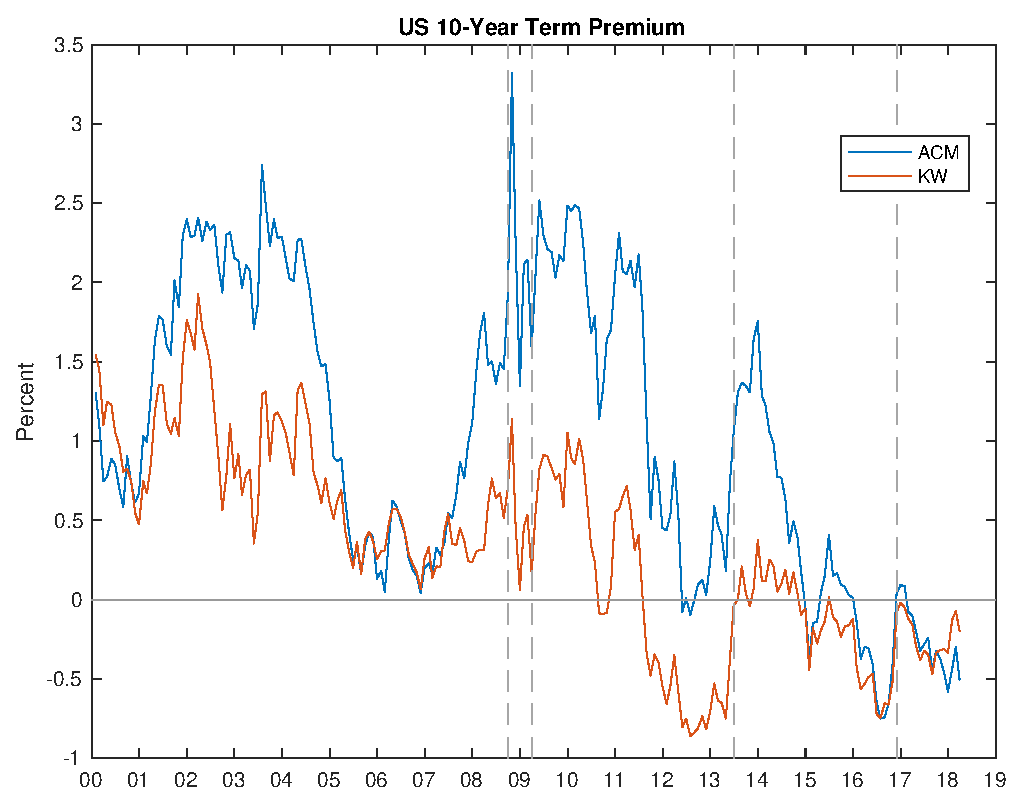
\includegraphics[width=0.9\textwidth,height=0.65\textheight]{../Figures/rp_us_10yr_ACMvsKM}
			\par\end{center}
		\caption{10-Year US Term Premium.}\label{fig:tp_us_10yr}
	\end{figure}}
\end{frame}
\note{Benchmark to compare how EM TPs behave.}
\note{Two frequently cited estimates of the US TP: KW and ACM.}
\note{Highlight three things: (1) the US TP is not constant; (2) it has decline over time; and (3) it has changed sign in recent years.}
\note{Explanations for decline: global investors, UMP.}
\note{Another explanation proposed by Campbell, Sunderam \& Viceira (2016) is that TP < 0 is explained by the flip in the sign of the correlation between stocks and bonds -bonds hedge stocks-.}
\note{We can analyze the behavior of the TP around key dates.}
\note{Vertical lines: September 2008, March 2009, June 2013, November 2016.}

\begin{frame}[label=tp_10yrA]
	\frametitle{Term Premium Estimates}
	\begin{figure}[!htbp]
		\begin{center}
			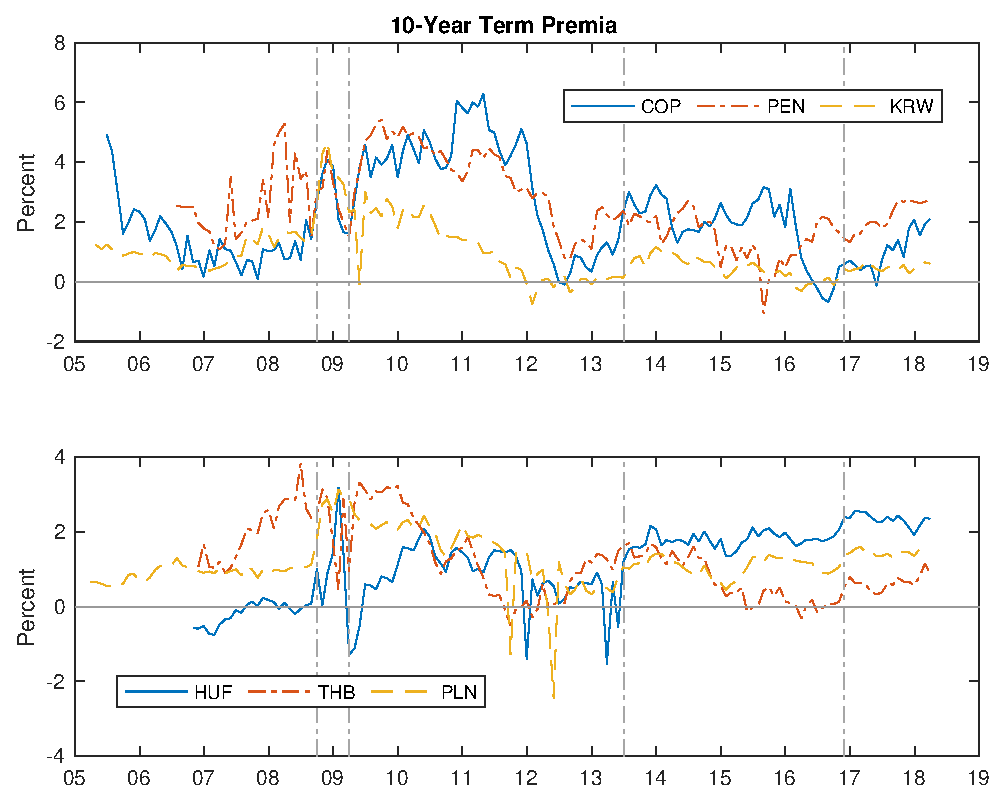
\includegraphics[width=0.9\textwidth,height=0.65\textheight]{../Figures/rp_10yr_1}
			\par\end{center}
		\caption{Estimated 10-Year Term Premia.}\label{fig:tp_10yrA}
	\end{figure}
	\begin{textblock*}{3cm}(.97\textwidth,-.08\textheight)
		\hyperlink{tp_10yrB}{\beamergotobutton{B}}
	\end{textblock*}
\end{frame}
\note{EM TP are time-varying.}
\note{Sensible TP estimates, mostly positive; fluctuate around 1\% and 2\%.}
\note{Sometimes they comove.}
\note{Behavior around vertical lines}
%\note{No same pattern to US TP seen in EMs}

\begin{frame}
	\frametitle{Term Structure of Term Premia}
	\begin{figure}[!htbp]
		\begin{center}
			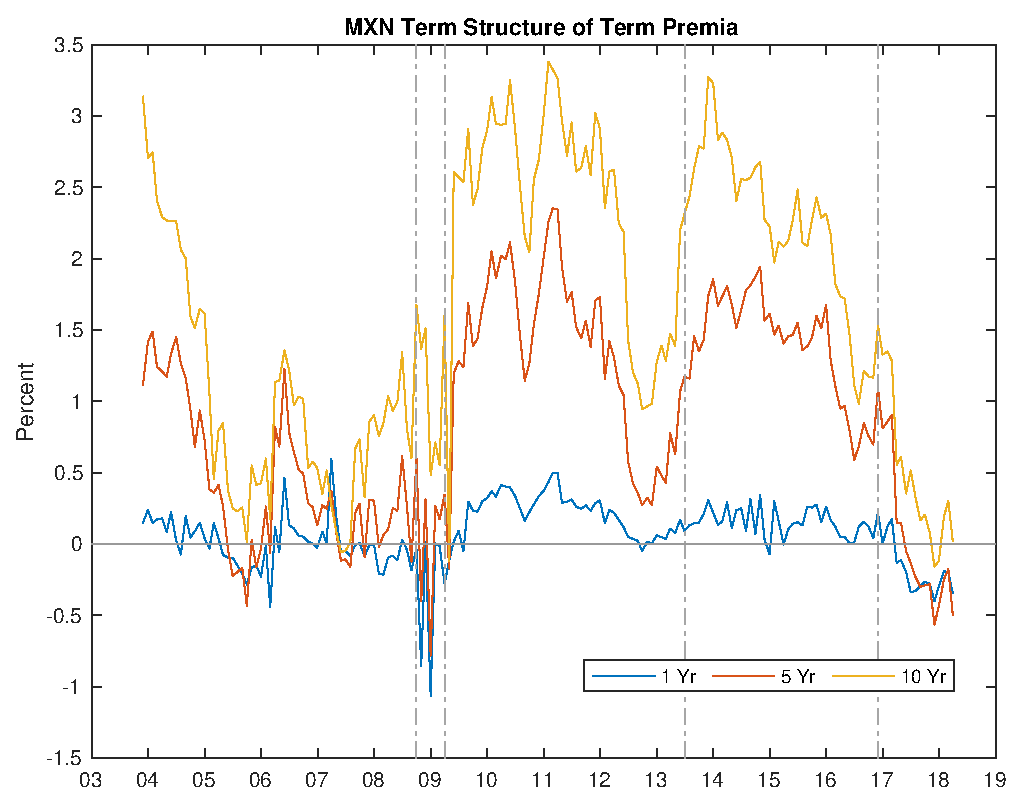
\includegraphics[width=0.9\textwidth,height=0.65\textheight]{../Figures/rp_ts_MXN}
			\par\end{center}
		\caption{Estimated 1-, 5- and 10-Year Term Premia.}\label{fig:tp_ts}
	\end{figure}
\end{frame}
\note{One can not only compare the TP across country but across maturities.}
\note{TP increases with maturity. As one would expect when LT are seen as risky, LT requiring a higher compensation.}
\note{Sometimes, standard deviation of TP increases with maturity.}

\begin{frame}
	\frametitle{Gains from `Adjusting' for Default Risk}
	\visible<2>{
	\begin{figure}[!htbp]
		\begin{center}
			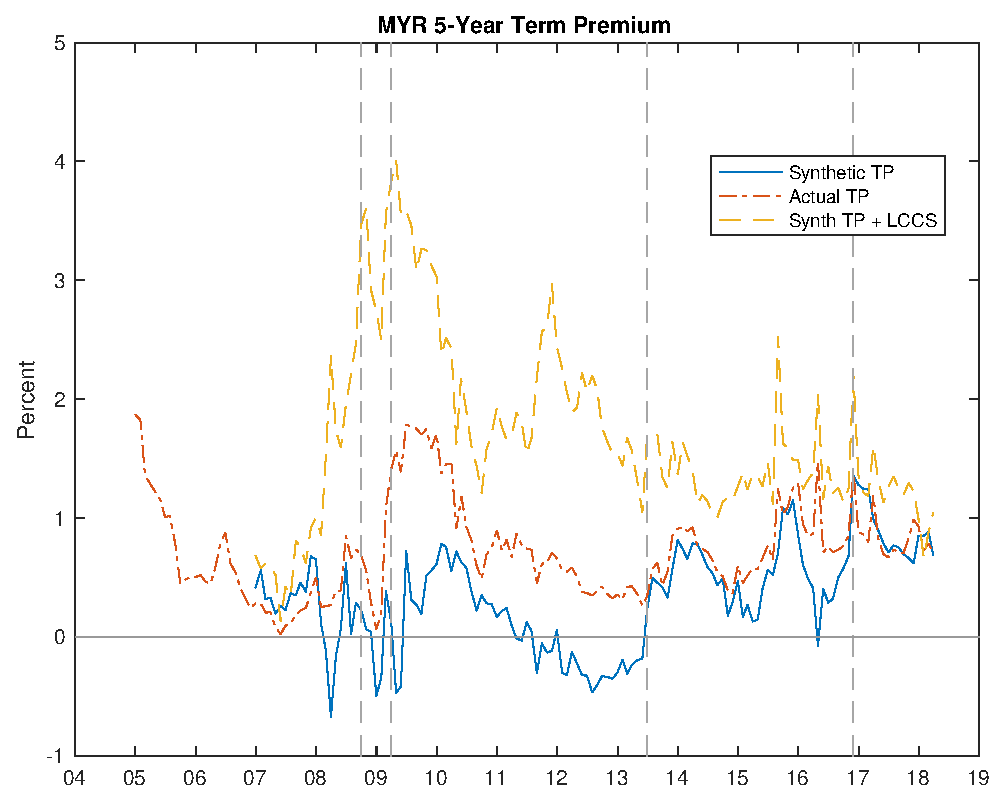
\includegraphics[width=0.9\textwidth,height=0.65\textheight]{../Figures/rp_cmp_5_MYR}
			\par\end{center}
		\caption{Estimated Term Premium: Synthetic vs Actual.}\label{fig:tp_comp_5yr}
	\end{figure}}
\end{frame}
\note{Explain each line.}
\note{Risk premium =! Term premium.}
\note{The dyanmics of TP and LCCS play an important role in EM bond yields.}

\begin{frame}
	\begin{tiny}\begin{table}\centering\begin{tabular}{l|cccccc}\toprule & N & Actual & Synthetic & Expected & TP & LCCS \\\midrule BRL & 141 & - & 8.55 & 7.00 & 1.55 & - \\COP & 154 & 8.82 & 7.09 & 4.90 & 2.19 & 1.06 \\HUF & 138 & 6.60 & 4.45 & 3.33 & 1.12 & 1.54 \\IDR & 205 & 9.36 & 9.31 & 8.39 & 0.92 & 0.73 \\ILS & 146 & 4.61 & 3.45 & 1.46 & 2.00 & 0.75 \\MXN & 173 & 7.51 & 7.00 & 5.36 & 1.64 & 0.33 \\PEN & 141 & 6.00 & 5.47 & 2.94 & 2.53 & 0.46 \\PHP & 219 & 7.94 & 7.41 & 5.57 & 1.84 & 0.76 \\PLN & 157 & 5.75 & 3.89 & 2.66 & 1.23 & 0.79 \\TRY & 155 & 10.97 & 10.34 & 10.87 & -0.53 & 0.57 \\KRW & 219 & 4.60 & 3.54 & 2.48 & 1.06 & 1.03 \\MYR & 136 & 4.24 & 3.21 & 2.33 & 0.88 & 0.77 \\RUB & 144 & 8.38 & 8.24 & 8.11 & 0.13 & 0.07 \\THB & 137 & 4.08 & 2.94 & 1.73 & 1.20 & 0.63 \\ZAR & 218 & 9.10 & 8.83 & 7.80 & 1.03 & 0.21 \\\bottomrule\end{tabular}\caption{LC Decomposition, 10-Year: Average Values.}\label{table:Decomp10yr}\end{table}\end{tiny}
\end{frame}
\note{Main component is expectation part. Mean and std of TP are higher than for LCCS.}
\note{It would be interesting to further decompose the nominal parts (Expected and TP) into real and inflation!!!}
\note{Mean: 6.9971    6.2480    4.9953    1.2527    0.6932}
\note{Std:    1.9943    1.8840    1.9940    1.1793    0.7597}

\begin{frame}
	\frametitle{Correlations}
	\begin{itemize}
		\item Comparison with US term premium
		\item LC credit spread (Du \& Schreger, 2016)
		\item Uncertainty indexes (Baker, Bloom \& Davis, 2016)
	\end{itemize}
\end{frame}
\note{EPU index is based on frequency of key words -economy, uncertainty, Fed- in newspapers. Only available for 5 countries in the sample.}

\begin{frame}[label=corr_10yr]
	\begin{tiny}\begin{table}\centering\begin{tabular}{l|ccc}\toprule & US TP & LCCS & EPU \\\midrule BRL & 0.38 & - & -0.29 \\COP & 0.67 & 0.09 & 0.13 \\HUF & 0.01 & -0.27 & - \\IDR & 0.36 & -0.21 & - \\ILS & 0.75 & -0.16 & - \\MXN & 0.72 & 0.20 & -0.05 \\PEN & 0.63 & -0.34 & - \\PHP & 0.49 & -0.22 & - \\PLN & 0.58 & -0.12 & - \\TRY & 0.76 & -0.16 & - \\KRW & 0.59 & 0.02 & -0.07 \\MYR & 0.23 & -0.53 & - \\RUB & 0.46 & -0.46 & -0.47 \\THB & 0.57 & -0.76 & - \\ZAR & 0.21 & 0.15 & - \\\bottomrule\end{tabular}\caption{Correlations of 10-Year Term Premia.}\label{table:Correls10yr}\end{table}\end{tiny}
	\begin{textblock*}{3cm}(.9\textwidth,-.5\textheight)
		\hyperlink{corr_5yr}{\beamergotobutton{5YR}}
	\end{textblock*}
\end{frame}
\note{EM TP and US TP are closely related, it tends to increase with maturity.}
\note{Correlation with LCCS is negative. Possible explanation: LCCS low reaction to global variables while the TP's is high.}
\note{For EPU, need to study BRL and RUB more closely. Note that for COP is positive.}

\begin{frame}
	\frametitle{Common Factors in EM Term Premia}
	\begin{footnotesize}\begin{table}\centering\begin{tabular}{l|cccc}
\toprule
\multicolumn{1}{c}{} &\multicolumn{2}{c}{EM TP}&\multicolumn{2}{c}{Residual}\\
\cmidrule(l{1.1em}r{1.1em}){2-3} \cmidrule(l{1.1em}r{1.1em}){4-5}
\multicolumn{1}{c}{} & 5 YR & 10 YR & 5 YR & 10 YR \\
\midrule
(15) Dec-06 & 67.40 & 71.67 & 62.99 & 58.25 \\(8)  Jul-05 & 79.57 & 82.65 & 74.36 & 76.40 \\(4)  Latam & 95.43 & 94.96 & 94.01 & 92.47 \\(5)  Asia & 90.19 & 91.43 & 88.52 & 87.98 \\(4)  Europe & 97.38 & 95.25 & 97.15 & 93.38 \\\bottomrule\end{tabular}\caption{Percent of Total Variance Explained by First 3 PCs.}\label{table:CmnFctrs}\end{table}\end{footnotesize}
\end{frame}
\note{Both domestic and common factors seem to be at play in EM TP.}

\begin{frame}
	\frametitle{Drivers of EM Term Premia}
	\begin{itemize}
		\item Panel regressions per maturity
		\item Global financial variables
		\begin{itemize}
			\item<2> VIX, Fed funds rate, S\&P, oil price
		\end{itemize}
		\item Domestic variables
		\begin{itemize}
			\item<2> Macro: Inflation, unemployment rate, industrial production
			\item<2> Financial: FX, stock market
		\end{itemize}
	\end{itemize}
\end{frame}

\begin{frame}[label=pnl_tp10yr]
	\frametitle{Panel Regression: 10-Year TP}
	{\centering
	\begin{tiny}\begin{tabular}{cccccc}
\toprule
log(VIX)& 0.021&-0.195&& 0.538***& 0.513***\\\
 &(0.33)&(0.32)&&(0.15)&(0.14)\\\
FFR&-0.198***& 0.009&&-0.149*& 0.109\\\
 &(0.08)&(0.08)&&(0.08)&(0.09)\\\
USTP10&& 0.546***&&& 0.639***\\\
 &&(0.06)&&&(0.06)\\\
SPX&-0.001***&-0.000&&-0.001***&\\\
 &(0.00)&(0.00)&&(0.00)&\\\
INF&&&-0.090&-0.136**&-0.150**\\\
 &&&(0.07)&(0.06)&(0.05)\\\
UNE&&& 0.160& 0.047& 0.029\\\
 &&&(0.12)&(0.10)&(0.09)\\\
IP&&&-0.008& 0.002&-0.001\\\
 &&&(0.01)&(0.01)&(0.01)\\\
Country FE&Yes&Yes&Yes&Yes&Yes\\\
Observations&2483&2483&1757&1757&1757\\\
Countries&15&15&15&15&15\\\
Within $R^2$&0.15&0.23&0.07&0.26&0.38\\\
\end{tabular}
\end{tiny} \par}
	\begin{textblock*}{3cm}(.92\textwidth,-.955\textheight)
		\hyperlink{pnl_tp5yr}{\beamergotobutton{5YR}}
	\end{textblock*}
\end{frame}
\note{Main broad message at 10 years. Big difference: FFR more negative when there is no USTP and disappears when USTP}
\note{Country fixed-effects were included to allow for the possibility that country-specific factors that may affect TP are also correlated with the controls.}

\begin{frame}
	\frametitle{Work in Progress}
	\begin{itemize}
		\item Given potential for small sample problems, use survey forecasts to discipline the model
		\begin{itemize}
			\item Key factor explaining differences in term premium estimates (Li, Meldrum \& Rodriguez, 2017)
		\end{itemize}
	\item Better characterization of EM term premia relative to AEs
	\end{itemize}
\end{frame}
\note{Next things on the list.}
\note{There is clearly uncertainty in the TP estimates and that is where survey forecasts can be helpful.}
\note{Identify more clearly where and how EM TPs differ from AEs. Broaden the number of AEs in the sample.}

\begin{frame}
	\frametitle{Work Ahead}
	\begin{itemize}
		\item Full implementation of ATSM to refine TP estimation
		\item Compare EMs with SOE AEs (Australia, NZ, Canada)
		\item Multi-country ATSM
		\pause
		\item Related work:
		\begin{itemize}
			\item Role of capital flows: negative EM TP?
			\item Role of FC yield curve: $\pi$ and FX expectations?
			\item High-frequency effects of MP on EM \textit{risk-free} yields
		\end{itemize}
	\end{itemize}
\end{frame}
\note{MP: US and local}

\section{Conclusions}

\begin{frame}
	\frametitle{Conclusions}
	\begin{itemize}
		\item `Clean' EM TP estimates using synthetic LC yield curves
		\begin{itemize}
			\item Gains from `adjusting' for credit risk
			\item In EMs, risk premium $\neq$ term premium
			\item More disaggregated decomposition of LC yield curves
		\end{itemize}
		\item Properties of EM term premia
		\item Many potential extensions
	\end{itemize}
\end{frame}


\section{Appendix}

\begin{frame}
	\begin{center}
		\huge \textcolor{yaleblue}{Appendix}
	\end{center}
\end{frame}

\begin{frame}
\frametitle{Benchmark}
\begin{figure}[!htbp]
	\begin{center}
		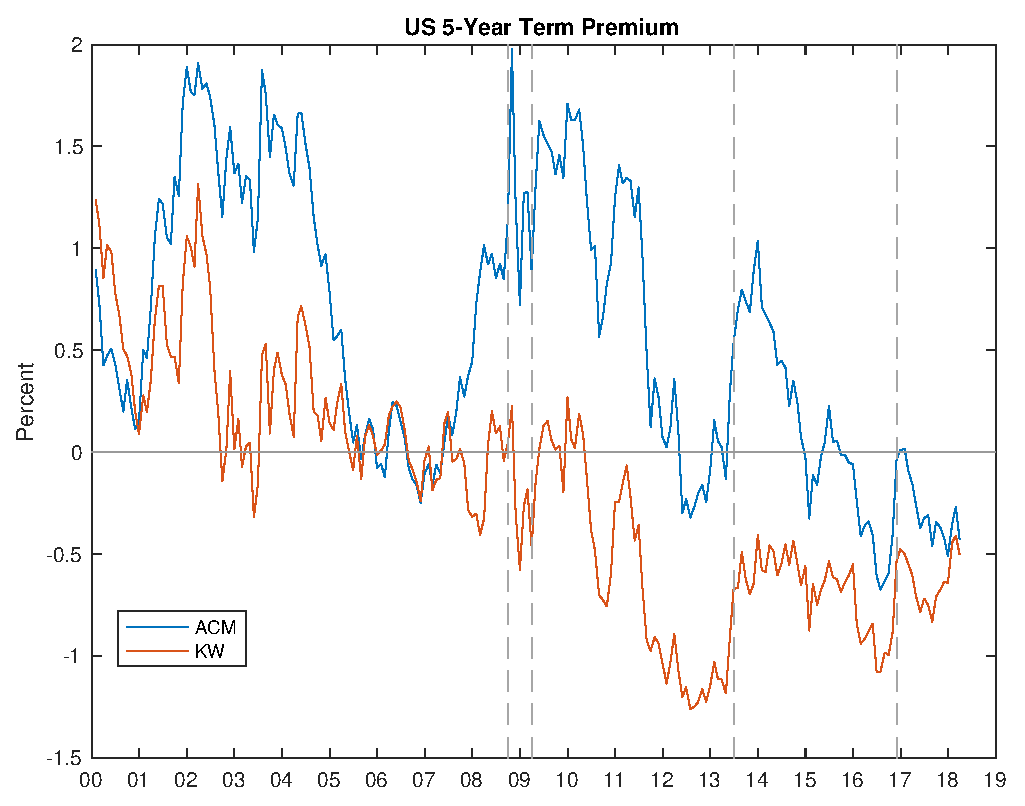
\includegraphics[width=0.9\textwidth,height=0.65\textheight]{../Figures/rp_us_5yr_ACMvsKM}
		\par\end{center}
	\caption{5-Year US Term Premium.}\label{fig:tp_us_5yr}
\end{figure}
\end{frame}

\begin{frame}[label=tp_10yrB]
	\frametitle{Term Premium Estimates}
	\begin{figure}[!htbp]
		\begin{center}
			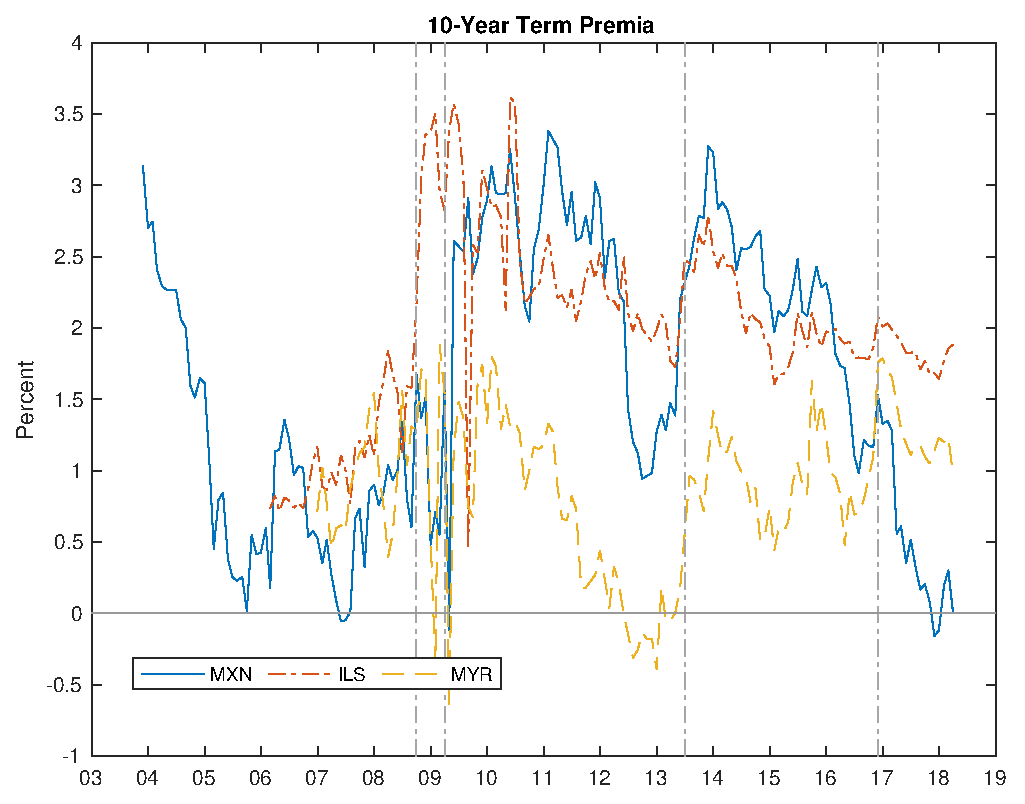
\includegraphics[width=0.9\textwidth,height=0.65\textheight]{../Figures/rp_10yr_3}
			\par\end{center}
		\caption{Estimated 10-Year Term Premia (cont.).}\label{fig:tp_10yrB}
	\end{figure}
	\begin{textblock*}{3cm}(.97\textwidth,-.08\textheight)
		\hyperlink{tp_10yrA}{\beamerreturnbutton{A}}
	\end{textblock*}
\end{frame}

\begin{frame}
	\frametitle{Term Premium Estimates}
	\begin{figure}[!htbp]
		\begin{center}
			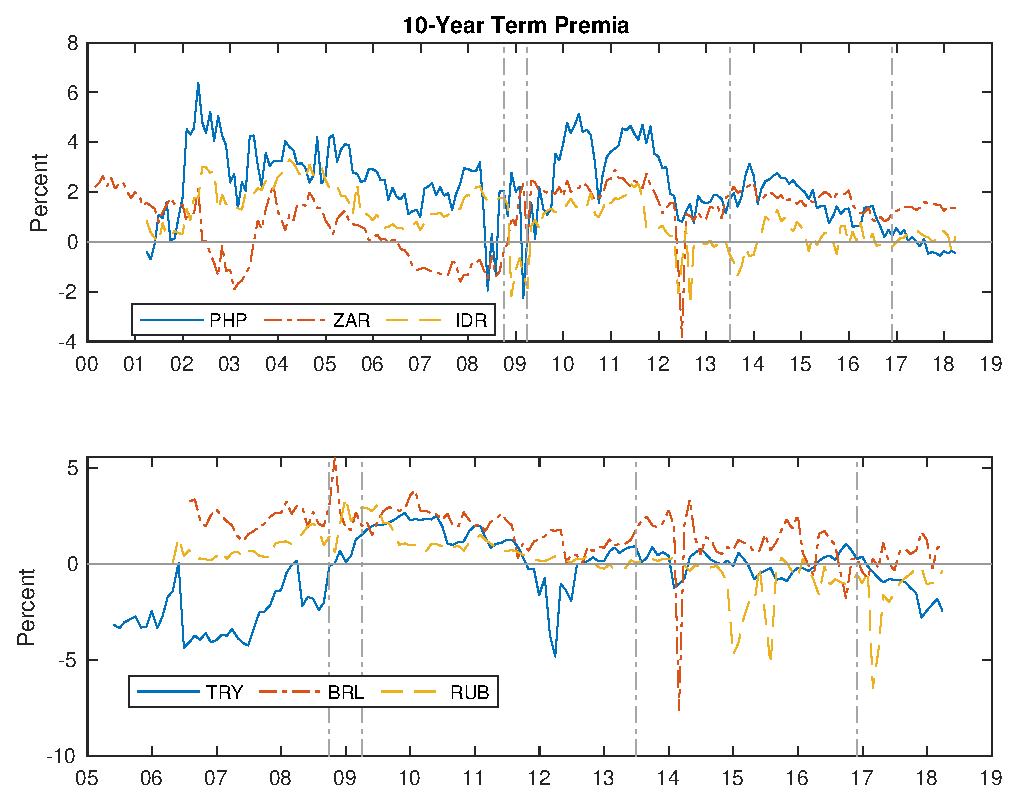
\includegraphics[width=0.9\textwidth,height=0.65\textheight]{../Figures/rp_10yr_2}
			\par\end{center}
		\caption{Estimated 10-Year Term Premia (cont.).}\label{fig:tp_10yrC}
	\end{figure}
	\begin{textblock*}{3cm}(.97\textwidth,-.08\textheight)
		\hyperlink{tp_10yrA}{\beamerreturnbutton{A}}
	\end{textblock*}
\end{frame}

\begin{frame}
	\frametitle{Gains from `Adjusting' for Default Risk}
	\begin{figure}[!htbp]
		\begin{center}
			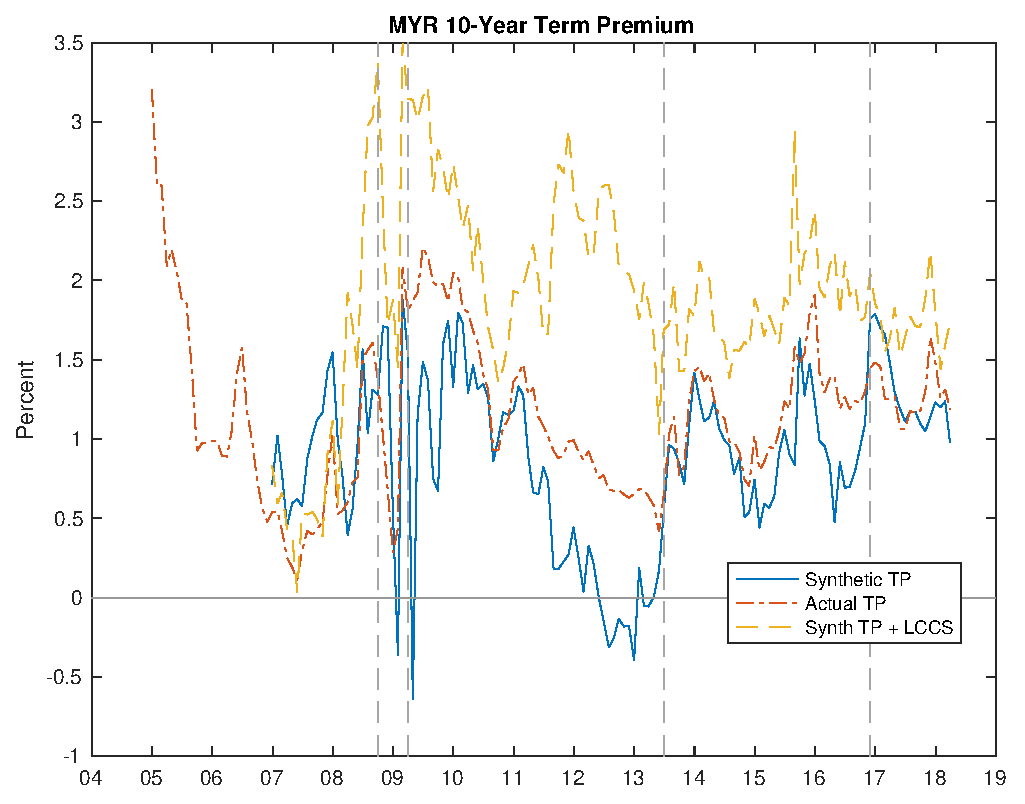
\includegraphics[width=0.9\textwidth,height=0.65\textheight]{../Figures/rp_cmp_10_MYR}
			\par\end{center}
		\caption{Estimated Term Premium: Synthetic vs Actual.}\label{fig:tp_comp_10yr}
	\end{figure}
\end{frame}

\begin{frame}
	\begin{tiny}\begin{table}\centering\begin{tabular}{l|cccccc}\toprule & N & Actual & Synthetic & Expected & TP & LCCS \\\midrule BRL & 141 & - & 8.64 & 7.05 & 1.59 & - \\COP & 154 & 8.21 & 6.22 & 4.92 & 1.31 & 1.39 \\HUF & 138 & 6.53 & 3.73 & 3.46 & 0.26 & 1.93 \\IDR & 205 & 8.89 & 8.97 & 8.48 & 0.49 & 0.66 \\ILS & 146 & 3.65 & 2.35 & 1.55 & 0.80 & 0.83 \\MXN & 173 & 6.91 & 6.22 & 5.35 & 0.87 & 0.56 \\PEN & 141 & 5.16 & 4.63 & 2.98 & 1.66 & 0.47 \\PHP & 219 & 7.14 & 6.55 & 5.66 & 0.89 & 0.88 \\PLN & 157 & 5.67 & 3.33 & 2.71 & 0.63 & 1.02 \\TRY & 155 & 11.71 & 10.52 & 10.88 & -0.35 & 0.63 \\KRW & 219 & 4.31 & 3.00 & 2.53 & 0.46 & 1.30 \\MYR & 136 & 3.74 & 2.67 & 2.33 & 0.33 & 0.98 \\RUB & 144 & 8.06 & 7.87 & 8.10 & -0.23 & 0.11 \\THB & 137 & 3.42 & 2.40 & 1.78 & 0.63 & 0.68 \\ZAR & 218 & 8.68 & 8.38 & 7.85 & 0.54 & 0.27 \\\bottomrule\end{tabular}\caption{LC Decomposition, 5-Year: Average Values.}\label{table:Decomp5yr}\end{table}\end{tiny}
\end{frame}

\begin{frame}[label=corr_5yr]
	\begin{tiny}\begin{table}\centering\begin{tabular}{l|ccc}\toprule & US TP & LCCS & EPU \\\midrule BRL & 0.20 & - & 0.12 \\COP & 0.61 & 0.43 & 0.08 \\HUF & 0.10 & -0.46 & - \\IDR & 0.17 & 0.35 & - \\ILS & 0.26 & -0.05 & - \\MXN & 0.62 & 0.15 & -0.14 \\PEN & 0.49 & 0.06 & - \\PHP & 0.40 & 0.17 & - \\PLN & 0.41 & 0.03 & - \\TRY & 0.79 & -0.26 & - \\KRW & 0.49 & 0.30 & -0.07 \\MYR & 0.07 & -0.62 & - \\RUB & 0.12 & -0.32 & -0.46 \\THB & 0.53 & -0.35 & - \\ZAR & 0.20 & 0.21 & - \\\bottomrule\end{tabular}\caption{Correlations of 5-Year Term Premia.}\label{table:Correls5yr}\end{table}\end{tiny}
	\begin{textblock*}{3cm}(.9\textwidth,-.5\textheight)
		\hyperlink{corr_10yr}{\beamerreturnbutton{10YR}}
	\end{textblock*}
\end{frame}

\begin{frame}[label=pnl_tp5yr]
	\frametitle{Panel Regression: 5-Year TP}
	{\centering
	\begin{tiny}\begin{tabular}{cccccc}
\toprule
log(VIX)&-0.284&-0.337&& 0.299**& 0.481**\\\
 &(0.32)&(0.31)&&(0.14)&(0.19)\\\
FFR&-0.157*&-0.024&&-0.061& 0.135\\\
 &(0.08)&(0.08)&&(0.08)&(0.08)\\\
USTP5&& 0.499***&&& 0.754***\\\
 &&(0.06)&&&(0.08)\\\
SPX&-0.001*&-0.000&&-0.001***&\\\
 &(0.00)&(0.00)&&(0.00)&\\\
INF&&&-0.096*&-0.138**&-0.136***\\\
 &&&(0.05)&(0.05)&(0.04)\\\
UNE&&& 0.153& 0.069& 0.072\\\
 &&&(0.1)&(0.08)&(0.07)\\\
IP&&&-0.005&-0.002& 0.001\\\
 &&&(0.01)&(0.01)&(0.01)\\\
Country FE&Yes&Yes&Yes&Yes&Yes\\\
Observations&2483&2483&1757&1757&1757\\\
Countries&15&15&15&15&15\\\
Within $R^2$&0.08&0.13&0.08&0.20&0.28\\\
\end{tabular}
\end{tiny} \par}
	%	\begin{tiny}\begin{table}\centering\begin{tabular}{cccccccc}\toprulelog(VIX) & -0.307*** & -0.134* &  &  0.275*** &  0.773*** &  0.772*** &  0.389*** \\\midrule  & (0.08) & (0.08) &  & (0.09) & (0.08) & (0.08) & (0.08) \\FFR & -0.162*** &  0.003 &  & -0.066*** & -0.089*** & -0.092*** &  0.071*** \\  & (0.01) & (0.02) &  & (0.02) & (0.02) & (0.02) & (0.02) \\USTP5 &  &  0.570*** &  &  &  &  &  0.679*** \\  &  & (0.04) &  &  &  &  & (0.04) \\SPX & -0.001*** &  &  & -0.001*** &  &  &  \\  & (0.00) &  &  & (0.00) &  &  &  \\INF &  &  & -0.096*** & -0.137*** & -0.112*** & -0.111*** & -0.130*** \\  &  &  & (0.01) & (0.01) & (0.01) & (0.01) & (0.01) \\UNE &  &  &  0.153*** &  0.068*** &  0.112*** &  0.111*** &  0.077*** \\  &  &  & (0.02) & (0.02) & (0.02) & (0.02) & (0.02) \\IP &  &  & -0.005 & -0.002 &  0.010** &  0.010** &  0.007* \\  &  &  & (0.00) & (0.00) & (0.00) & (0.00) & (0.00) \\Country FE & Yes & Yes & Yes & Yes & Yes & Yes & Yes \\Observations & 2483 & 2468 & 1757 & 1757 & 1752 & 1752 & 1752 \\Countries & 15 & 15 & 15 & 15 & 15 & 15 & 15 \\R-squared & 0.227 & 0.257 & 0.304 & 0.394 & 0.349 & 0.35 & 0.431 \\\bottomrule\end{tabular}\caption{Panel Regression: 5-Year TP.}\label{table:Panel5yr}\end{table}\end{tiny}
	\begin{textblock*}{3cm}(.92\textwidth,-.955\textheight)
			\hyperlink{pnl_tp10yr}{\beamerreturnbutton{10YR}}
	\end{textblock*}
\end{frame}

\end{document}

%---------------------------------------------------------------
% Sources
%---------------------------------------------------------------
% Tips in general
% https://en.wikibooks.org/wiki/LaTeX/Presentations
%https://tex.stackexchange.com/questions/12328/how-can-i-use-todonotes-with-beamer
% Insert links to slides
% https://latex.org/forum/viewtopic.php?t=4594
% Place button of link on slide
%https://tex.stackexchange.com/questions/50643/hyperlink-button-in-an-exact-position
% Make figures visible
%https://stackoverflow.com/questions/4683093/beamer-how-to-show-images-as-step-by-step-images
% Multicolumn and multirow
%https://tex.stackexchange.com/questions/156219/proper-centering-with-cmidrule-and-multi-row-and-column

% Code for hyperlinks
%[label=corr_10yr]
%\begin{textblock*}{3cm}(.9\textwidth,-.5\textheight)
%	\hyperlink{corr_10yr}{\beamergotobutton{10-Year TP}}
%\end{textblock*}
%
%\begin{textblock*}{3cm}(.9\textwidth,-.5\textheight)
%	\hyperlink{corr_10yr}{\beamerreturnbutton{10-Year TP}}
%\end{textblock*}